% chapter 2
\chapter{Theory}
Before we proceed the actual content of the study, it is useful to introduce some theories that will help the reader
to understand the concepts mentioned in the rest of this project. In this section, we will discuss the basics of
linear programming and basic algorithms used for solving them. We will
also discuss briefly how constraints programming is implemented in linear programming solver software.

\section{Linear Programming}
Linear programming is a mathematical method that is commonly used to retrieve an optimal solution from model
that has been converted into a linear system. This model is achieved when all of the mathematical relationship in the model
uses linear functions exclusively. The word 'programming' is not to be confused with the term used in computer science,
in which concerns with formulating instructions for computers to execute. A linear programming system (also called linear
program) consists of three entities:
\begin{enumerate}
\item \textbf{Decision variables} - These are the entities that can be controlled by the decision maker.
\item \textbf{Objective function} - This is the function that, given the optimal input, outputs the optimal value.
In most cases, it is to find the minimum or the maximum value.
\item \textbf{Variable constraints} - These are the restrictions that are imposed on the decision variables. There are two types
of constraints: hard and soft. Hard constraints are constraints cannot be violated at all cost, whereas soft constraints may be
violated, but should be observed wherever possible.
\end{enumerate}
To further undestand how this works, let's walk through a simple example: Bob is competing in
an eating contest where the objective is to accumulate as much points as possible by eating a combination of hotdogs and burgers.
For each burger and hotdog that Bob ate, he will get 5 and 4 points respectively. It takes him 3 minutes to finish a burger and
2 minutes to finish a hotdog and the contest lasts one hour. Bob can consume 25 food items before his appetite reaches its limit.

Based on the scenario above, we can model this problem in the form of a linear program by following these steps:
\begin{itemize}
\item \textbf{Step 1}: Identify the decision variables. Let \(x\) be the number of hotdogs and \(y\) be the number
of burgers eaten by Bob.
\item \textbf{Step 2}: Determine the objective function. In this scenario, we want to determine the highest possible
points that Bob can achieve in the competition. This can be represented by the equation \(z = 4x + 5y\), where
z is the value of the points accumulated in the competition and the coefficients of the variables represent the points achieved by eating respective
food items.
\item \textbf{Step 3}: Determine the constraints. There are 3 constraints in these problem. Firstly, The amount of
food eaten by bob has to be under 60 minutes. This can be represented by the equation \(2x + 3y \leq 60\). Secondly,
Bob's appetite has a limit of 25 food items, which can be modelled with the equation \(x + y \leq 25\). Lastly,
the number of respective food eaten has to be greater than or equal to 0.
\end{itemize}
Putting it together, we have the following linear program:
\[
  \begin{array}{r@{}r@{}l}
    \text{Maximise z =} \quad &{}4x + 5y \\[\jot]
    \text{Subject to}\qquad &{} 2x +   3y &{} \leq 60 \\
    \qquad &{} x +   \phantom{2}y &{} \leq 25 \\
    \qquad &{} x ,   \phantom{2}y &{} \geq 0 \\
  \end{array}
\]
There are two types of solution that can be produced. A feasible solution is a set of variables that satisfies the constraints
of a linear program. An example of a feasible solution for the above solution would be \(x = 25\) and \(y=0\), which yields 100 points.
Optimal solution is the best feasible solution, such as when \(x = 15\) and \(y = 10\), which gives 110 points. In all cases, we want to
find the \textit{optimal} solution. Also, There are 3 types of outcomes in a linear program:

\begin{itemize}
\item \textbf{Outcome 1} : The feasible region is unbounded, thus the objective function is infinity.
\item \textbf{Outcome 2} : The feasible region is empty, this is usually because the constraints on the variables contradict each other.
\item \textbf{Outcome 3} : There is a feasible region that is also bounded. In this case, an optimal solution exists!
\end{itemize}

\begin{figure}[!ht]
  \centering
    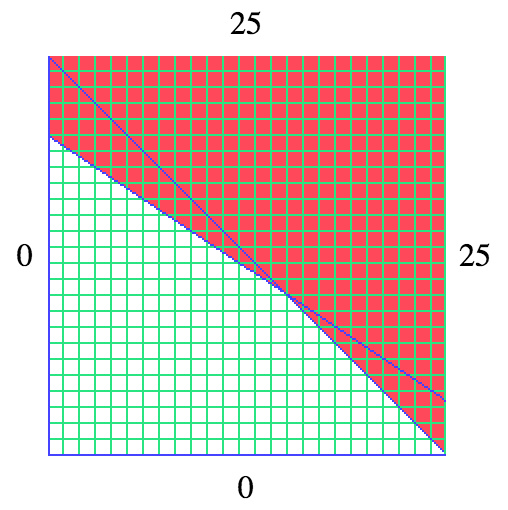
\includegraphics[width=0.5\textwidth]{example-graph.png}
    \caption{Graph representation of a linear program example. The feasible region is shown in white. The optimal solution
  is located at the point (15,10).}
\end{figure}
In order to produce an optimal solution, we can use the simplex algorithm. To understand simplex algorithm, it is best to look at
a graphical representation of the linear program. The simplex algorithm starts off by selecting a point in a graph.
Then it moves to a different point of the graph. On each move, it will make sure that the point yield higher
objective value, by using the values of its axes. If no higher objective value is found, then that point would be the
optimal solution. This method also works in higher dimensional spaces. This explanation is just a simplication of the full
simplex algorithm. The reader may refer to the references section resources that explains the algorithm in detail.

\begin{figure}[!ht]
  \centering
    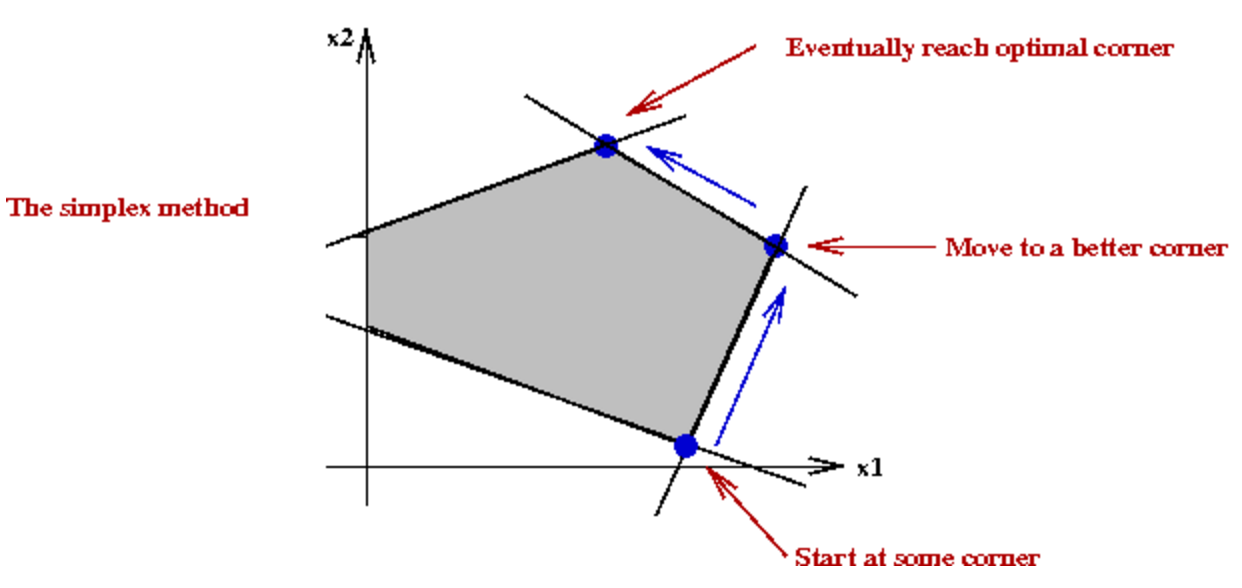
\includegraphics[width=1\textwidth]{simplex.png}
    \caption{Simplex method on a linear program}
\end{figure}

The number of variables in the linear program correspond to the number of dimensions in its graphical representation. For example,
a linear program with 3 variables could be represented by the polyhedra below:

\begin{figure}[!ht]
  \centering
    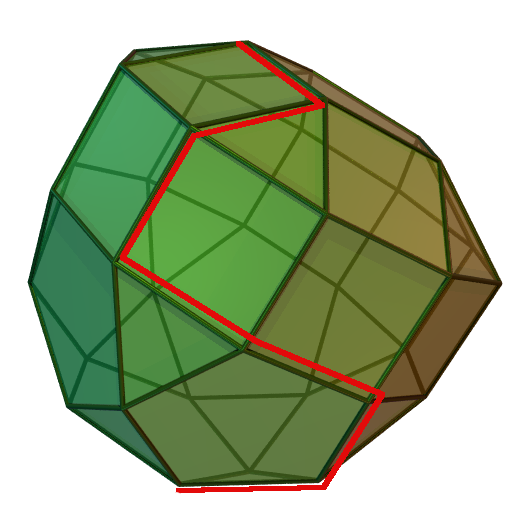
\includegraphics[width=0.4\textwidth]{simplex3d.png}
    \caption{Simplex algorithm on a polyhedra}
    \vspace{1cm}
    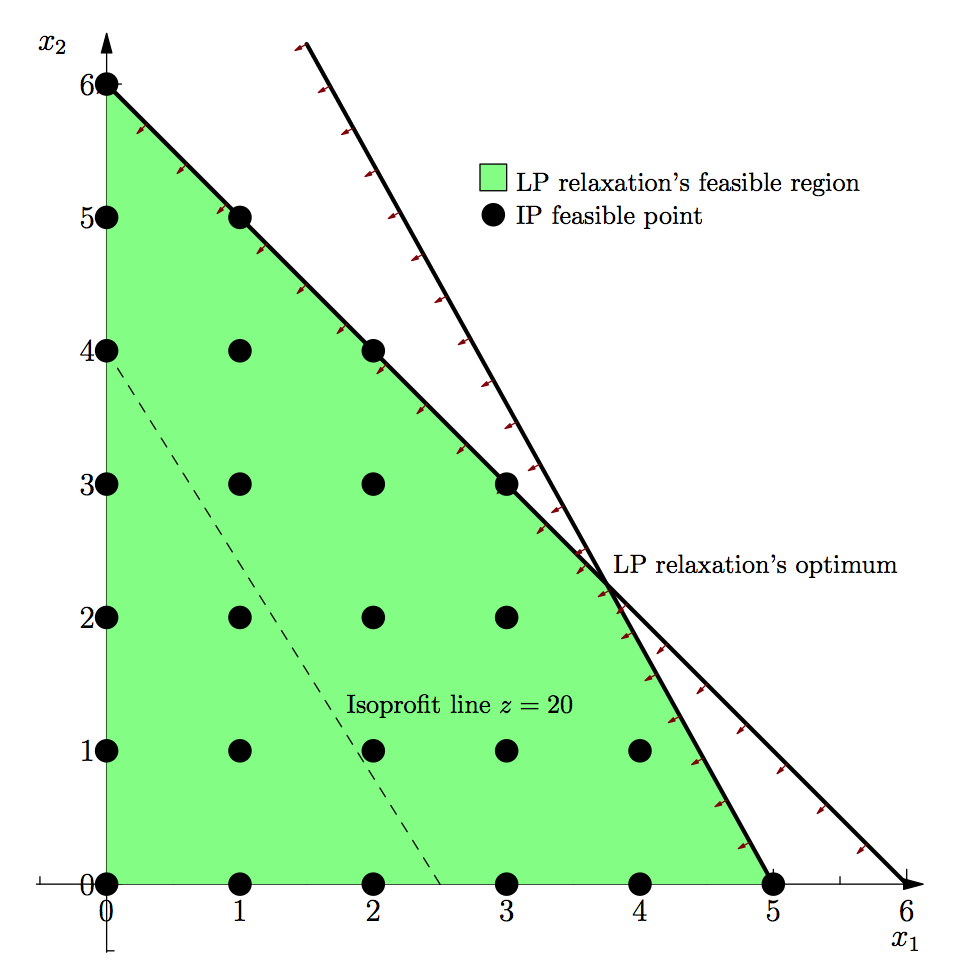
\includegraphics[width=0.7\textwidth]{ipfeasible.png}
    \caption{A graphical representation of a hypothetical linear program. The region bounded by the black line
  line represent the feasible region of the linear program. The region bounded by the blue line represent
   the feasible region of the same linear program, with the addition of itegrality constraint imposed into it.}
\end{figure}

\section{Integer Programming}
Integer programming (also known as integer linear programming) is a system where a linear program has an additional
integrality constraint of imposed on to its decision variables. This is useful in situations where real or
fractional valued variables are not realistic, such as the number of people that it takes to complete a task or the
length of the tour in a hamiltonian cycle.
When this constraint is added, finding an optimal solution becomes harder. This is because the solution can only be
in the lattice points of the graph, thereby
reducing the solution space. Linear programming in which only some of the variables have integrality constraints imposed
into it is known as mixed integer programming (MIP).

More sophisticated algorithms have been invented in order to accomodate the added complexity of IP. One of the most commonly
used algorithm that produces the exact solution is the branch and bound algorithm. It is uses divide and
conquer approach to partition the problem into sub-problems
and then solves them recursively. LP methods such as the simplex can be used to solve the sub-problems.
There are 2 parts to the algorithm: branch and bound. The 'branching' part generates a tree
that continues to expand until all valid solutions are found. The bound part compares all solutions and keeps the
most optimal one.

Let's look at an example to see how it works:
\[
  \begin{array}{r@{}r@{}l}
    \text{Maximise} \quad &{}x_{1} + 12x_{2} \\[\jot]
    \text{subject to}\qquad &{}10x_{1} +   7x_{2} &{} \leq 40 \\
    \qquad &{} x_{1} +   \phantom{2}x_{2} &{} \leq 5 \\
    \qquad &{} x_{1} ,   \phantom{2}x_{2} &{} \in \mathbb{Z}_{>0}\\
  \end{array}
\]

These are the steps of the branch of bound algorithm as it solves the IP problem above:
\begin{itemize}
\item The 'branch' part:
    \begin{itemize}
        \item \textbf{Step 1} : We start by solving the given ILP problem using standard LP method such as the simplex algorithm. Then, we pick the
         variables that does not conform to the integrality constraint as the branching variables. At this point, We are at the root of
         the tree that is generated by this algorithm.
        \item \textbf{Step 2} : Create 2 branches for the chosen branching variable and set a new constraints to that variable in those branches
        . For example, in the children of the root node of the figure 2.5,
         we impose the constraint \(x_{1} \leq 1\) on the left side and \(x_{1} \geq 2\) on the right side of the branch.
        \item \textbf{Step 3} : This is the recursive step of the branching algorithm. We pick a branch and then solve it
        using the same method in step 1. At this point, there are 3 possible outcomes:
            \begin{enumerate}
                \item Infeasible solution: the algorithm will not continue branching from this node and picks other unexplored node
                to solve.
                \item Integral solution found : the algorithm will stop here, record the solution and move on to solve other unexplored node.
                \item Fractional/real solution found: Choose a branching algorithm and then go back to step 2 of this part of the algorithm.
                Exit if there are no explored nodes left.
            \end{enumerate}
    \end{itemize}
\item The 'bound' part: The algorithm will compare all solutions found and keep the most optimal one. The optimal value is set negative infinity at first
and it will be immediately replaced as soon as an integral solution is found.
 This will give the exact solution of the problem.
\end{itemize}

\vspace{0.5cm}

\begin{figure}[!ht]
  \centering
    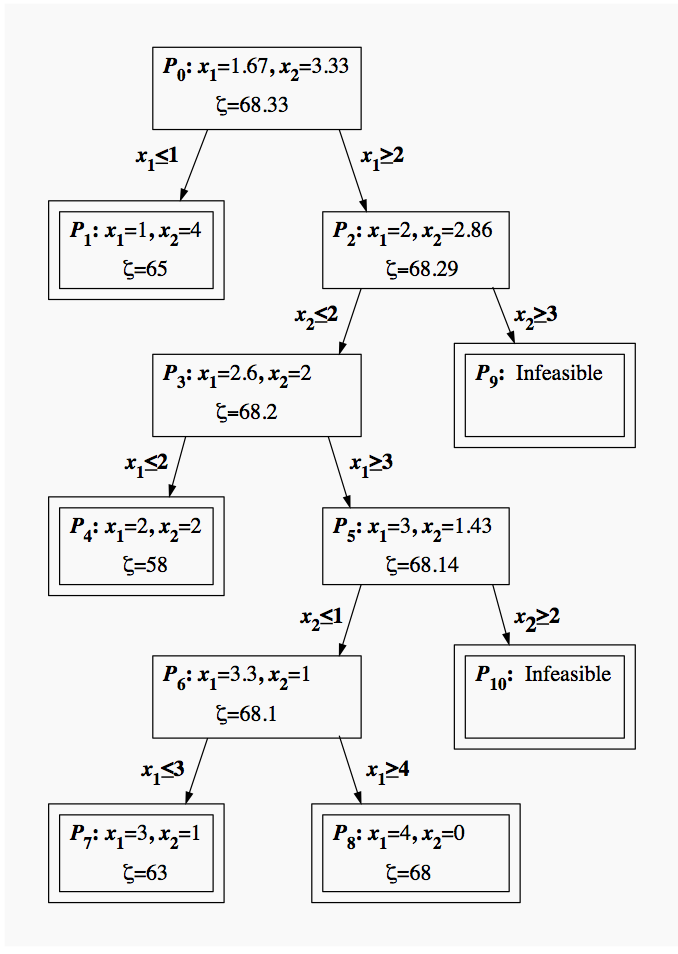
\includegraphics[width=0.6\textwidth]{BNB.png}
    \caption{Enumeration tree that is generated by the branch and bound algorithm for the sample IP problem}
\end{figure}

\section{Constraints Programming}
Unlike the programming that we have observed so far, constraints programming is a programming paradigm that is implemented
in linear programming solvers. Understanding the basics of constraints programming will give insights to how linear programming
solvers work under the hood.

Constraints programming (CP) is a programming paradigm that combines declarative and procedural paradigm. This seems contradictory
at first, because declarative formulation is static whereas a procedural one is dynamic. The idea is boiled down to viewing
a constraint the same way as invoking a procedure. The goal of CP is to find feasible solutions out of large solutions space, making it
more suitable to accomodate LP. Due to this goal, CP focuses on the constraints and variables rather than the objective function.

In this paradigm, a constraint program may be written declaratively but should be viewed as a procedure that operates on a
solution space. Each constraints will be added to a constraint store, which limits the space that must be searched.
Constraint store uses a filtering algorithm that serves as a litmus test for solutions. These solutions will be 'filtered'
by the constraints, which has become part of the constraint store. At the end of the filtering procedure, we obtain a feasible solution.

Given this view, constraint programming formulation tends to look
more like a mathematical programming model than a computer program, since the user writes constraints declaratively
rather than writing procedures to enforce these constraints. For this reason, CP is more suited for solving computer programs that are
LP-based.